\documentclass{report}
\usepackage{amssymb, amsmath}
\usepackage{graphicx}
\usepackage{float}

\title{Examen Segundo Parcial}
\date{20 de Octubre de 2022}
\author{Nestor Adrian Sandoval Ortiz}

\begin{document}
    \maketitle
    \chapter{Optimizacion deterministica sin restricciones}
        \paragraph{Introduccion}
        A continuacion se muestran 7 ejercicios correspondientes al segundo examen parcial de la
        materia de Optimizacion. Es importante destacar que, por cada problema, se realizaran 1000
        ejecuciones independientes con el fin de realizar un analisis y comparacion mas precisos entre
        distintos algoritmos.

        \pagebreak

        \section{Primer Ejercicio}
            \begin{equation*}
                f(x)=x^2exp(x)+y^2exp(y)+1 
            \end{equation*}

            \begin{figure}[H]
                \includegraphics[width=\linewidth]{/Users/lloydna/Projects/School/Optimizacion/Optimizacion/Examenes/Examen2/Ejercicio1/funcion.png}
                \caption{Grafica de la funcion y su minimo}
                \label{fig:fun11}
            \end{figure}

            \subsection{Tabla de resultados}
                \begin{tabular}{l|p{1.5cm}|p{1.5cm}|p{1.5cm}|p{1.5cm}|p{1.5cm}|p{1.5cm}}
                    & (x,y) Promedio & f(x,y) Promedio & Mejor (x,y) & Mejor f(x,y) & Peor (x,y) & Peor f(x,y)\\
                    \hline
                    Newton Raphson & (0.0, 0.0) & 1.0 & (0.0, 0.0) & 1.0 & (0.0, 0.0) & 1.0\\
                    \hline
                \end{tabular}

            \subsection{Interpretacion de resultados}
                El minimo global se ubica en el punto (0,0,1), esto se debe a que, si bien, la funcion exponencial
                nunca vale 0, los cuadrados de las variables si que lo hacen en 0, provocando que los terminos exponenciales
                se cancelen, dejando unicamente a la constante "1" como valor minimo de la funcion.
        \pagebreak

        \section{Segundo Ejercicio}
            \begin{equation*}
                f(x)=120+1.5x+\frac{0.2}{x}(1000) 
            \end{equation*}

            \begin{figure}[H]
                \includegraphics[width=\linewidth]{/Users/lloydna/Projects/School/Optimizacion/Optimizacion/Examenes/Examen2/Ejercicio2/funcion.png}
                \caption{Grafica de la funcion y su minimo}
                \label{fig:fun12}
            \end{figure}

            \subsection{Tabla de resultados}
                \begin{tabular}{l|c|c|c|c|c|c}
                    & x Promedio & f(x) Promedio & Mejor x & Mejor f(x) & Peor x & Peor f(x)\\
                    \hline
                    Newton Raphson & 11.54348 & 154.64102 & 11.54348 & 154.64102 & 11.54348 & 154.64102\\
                    \hline
                \end{tabular}

            \subsection{Interpretacion de resultados}
                Es sumamente curioso como la funcion que describe la eficiencia de este motor demuestra que no siempre lo que menos usa es "lo mejor"
                y es que, mientras la potencia mas se aleja de 1 y se acerca a 0, mas se dispara el precio a una velocidad increible.
        \pagebreak

        \section{Tercer Ejercicio}
            \begin{equation*}
                f(x)=x^2+x^4
            \end{equation*}

            \begin{figure}[H]
                \includegraphics[width=\linewidth]{/Users/lloydna/Projects/School/Optimizacion/Optimizacion/Examenes/Examen2/Ejercicio3/funcion.png}
                \caption{Grafica de la funcion y su minimo}
                \label{fig:fun13}
            \end{figure}

            \subsection{Tabla de resultados}
                \begin{tabular}{l|c|c|c|c|c|c}
                    & x Promedio & f(x) Promedio & Mejor x & Mejor f(x) & Peor x & Peor f(x)\\
                    \hline
                    Newton Raphson & -0.0 & 0.0 & -0.0 & 0.0 & -0.0 & 0.0\\
                    \hline
                    Secante & -0.01295 & 0.00017 & -0.01295 & 0.00017 & -0.01295 & 0.00017\\
                    \hline
                \end{tabular}
            
            \subsection{Interpretacion de resultados}
                Justo en esta comparacion sale a relucir una de las mas grandes ventajas del metodo de
                Newton contra el de la Secante, y esque, mientras el metodo de la Secante REQUIERE que
                entre ambos puntos exista un minimo (de lo contrario, el algoritmo se queda en un ciclo sin fin),
                el de Newton solo requiere de una aproximacion inicial al minimo con la que establecera un camino
                de busqueda sin riesgos a entrar en un ciclo infinito.
                Por ultimo, cabe destacar que, por lo anteriormente mencionado, el algoritmo de la Secante NO funciona
                con los parametros iniciales en el problema, y, debido a esto, fue necesario cambiar el punto inicial "b"
                de -3 a 3.
        \pagebreak

        \section{Cuarto Ejercicio}
            \begin{equation*}
                f(x)=x^2+x^4
            \end{equation*}

            \begin{figure}[H]
                \includegraphics[width=\linewidth]{/Users/lloydna/Projects/School/Optimizacion/Optimizacion/Examenes/Examen2/Ejercicio3/funcion.png}
                \caption{Grafica de la funcion y su minimo}
                \label{fig:fun14}
            \end{figure}

            \subsection{Tabla de resultados}
                \begin{tabular}{l|c|c|c|c|c|c}
                    & x Promedio & f(x) Promedio & Mejor x & Mejor f(x) & Peor x & Peor f(x)\\
                    \hline
                    Newton Raphson & -0.0 & 0.0 & -0.0 & 0.0 & -0.0 & 0.0\\
                    \hline
                    Secante & -0.02276 & 0.00052 & -0.02276 & 0.00052 & -0.02276 & 0.00052\\
                    \hline
                \end{tabular}

            \subsection{Interpretacion de resultados}
            En esta ocasion a delta x se le asigno un valor de 0.01, culminando en unos resultados
            interesantes en donde el metodo de Newton sigue demostrando su superioridad sin mostrar
            diferencia aparente con su contraparte explicita (al menos en el rango de 5 decimales).
        \pagebreak

        \section{Quinto Ejercicio}
            \begin{equation*}
                f(x,y)=x^2+y^2-2x
            \end{equation*}

            \begin{figure}[H]
                \includegraphics[width=\linewidth]{/Users/lloydna/Projects/School/Optimizacion/Optimizacion/Examenes/Examen2/Ejercicio5/funcion.png}
                \caption{Grafica de la funcion y su minimo}
                \label{fig:fun15}
            \end{figure}

            \subsection{Tabla de resultados}
                \begin{tabular}{p{1.5cm}|p{1.5cm}|p{1.5cm}|p{1.5cm}|p{1.5cm}|p{1.5cm}|p{1.5cm}}
                    & (x,y) Promedio & f(x,y) Promedio & Mejor (x,y) & Mejor f(x,y) & Peor (x,y) & Peor f(x,y)\\
                    \hline
                    Newton Raphson (multidimensional) & (1.00001, 1.0e-5) & -1.0 & (1.00001, 1.0e-5) & -1.0 & (1.00001, 1.0e-5) & -1.0\\
                    \hline
                    Newton Raphson (unidimensional) & (1.0,0.0) & -1.0 & (1.0,0.0) & -1.0 & (1.0,0.0) & -1.0\\
                    \hline
                    Secante (unidimensional) & (1.0,0.0) & -1.0 & (1.0,0.0) & -1.0 & (1.0,0.0) & -1.0\\
                    \hline
                \end{tabular}

            \subsection{Interpretacion de resultados}
                Resulta bastante interesante que los metodos unidimensionales superaran al multidimensional por un poco,
                lo que da a entender que, en ciertas funciones, es mas conveniente minimizar variables individualmente con el
                fin de dividir un problema grande en sub-problemas chicos mas faciles de resolver.
        \pagebreak

        \section{Sexto Ejercicio}
            \begin{equation*}
                f(x,y)=(x+2y-7)^2+(2x+y-5)^2
            \end{equation*}

            \begin{figure}[H]
                \includegraphics[width=\linewidth]{/Users/lloydna/Projects/School/Optimizacion/Optimizacion/Examenes/Examen2/Ejercicio6/funcion.png}
                \caption{Grafica de la funcion y su minimo}
                \label{fig:fun16}
            \end{figure}

            \subsection{Tabla de resultados}
                \begin{tabular}{l|p{1.5cm}|p{1.5cm}|p{1.5cm}|p{1.5cm}|p{1.5cm}|p{1.5cm}}
                    & (x,y) Promedio & f(x,y) Promedio & Mejor (x,y) & Mejor f(x,y) & Peor (x,y) & Peor f(x,y)\\
                    \hline
                    Newton Raphson & (1.00001, 1.0e-5) & -1.0 & (1.00001, 1.0e-5) & -1.0 & (1.00001, 1.0e-5) & -1.0\\
                    \hline
                \end{tabular}
        \pagebreak

        \section{Septimo Ejercicio}
            \begin{equation*}
                f(X)=(100(X_{2}-X_{1}^2))^2+(1-X_{1})^2+90(X_{4}-X_{3}^2)^2+(1-X_{3})^2+10.1((X_{2}-1)^2+(X_{4}-1)^2)+19.8(X_{2}-1)(X_{4}-1)
            \end{equation*}

            \subsection{Tabla de resultados}
                \begin{tabular}{l|p{1.5cm}|p{1.5cm}|p{1.5cm}|p{1.5cm}|p{1.5cm}|p{1.5cm}}
                    & X Promedio & f(X) Promedio & Mejor (X) & Mejor f(X) & Peor (X) & Peor f(X)\\
                    \hline
                    Gradiente & (0.99141, 0.98288, 1.00851, 1.01712) & 0.00026 & (0.99141, 0.98288, 1.00851, 1.01712) & 0.00026 & (0.99141, 0.98288, 1.00851, 1.01712) & 0.00026\\
                    \hline
                \end{tabular}

            \subsection{Interpretacion de resultados}
                Observando los resultados, es intuitivo entender que el minimo de la funcion se ubica en las coordenadas (1,1,1,1,0).
                Se aplico el metodo del gradiente debido a su simplicidad (contrario al mas preciso pero complejo metodo de Newton),
                utilizando una tecnica multiarranque hasta dar con un punto adecuado que no dirigiera a valores gigantescos alejados de la solucion,
                este problema en particular resulto ser bastante demandante computacionalmente gracias a lo diminuta
                que tenia que ser la taza de aprendizaje (puesto que si era aunque sea unas milesimas mas grande, terminaba llevando al algoritmo a puntos muy alejados de la solucion),
                requiriendo un total de 1,000,000 de iteraciones para llegar a un resultado estable y aceptable.
        \pagebreak
        
\end{document}